\chapter{Introduction}
This project develops a lightweight web application using HTML5 \texttt{<video>} and Canvas for real-time edge detection. During playback, each displayed frame is processed locally in the browser using client-side JavaScript, and the resulting edge map is rendered alongside the original video.

\chapter{Guidance}
\section{Access}
\begin{itemize}
  \item \textbf{GitHub repository:} \url{https://github.com/ariesanhthu/homework5}
  \item \textbf{GitHub Pages:} \url{https://ariesanhthu.github.io/homework5/}
\end{itemize}

\section{Local setup}
To run the application locally, install the required dependencies, start the Node.js server, and open the local host address in a web browser.

\section{Usage}
The user can either select a local video file or load the bundled sample video. During playback, the interface presents two synchronized views: the original video and the corresponding edge map generated in real time on the Canvas. The page also provides a threshold mode selector (\emph{Manual} or \emph{Adaptive}) and a slider for tuning the high-threshold behavior. Processing stops automatically when playback is paused or completed.

\begin{figure}[H]
  \centering
  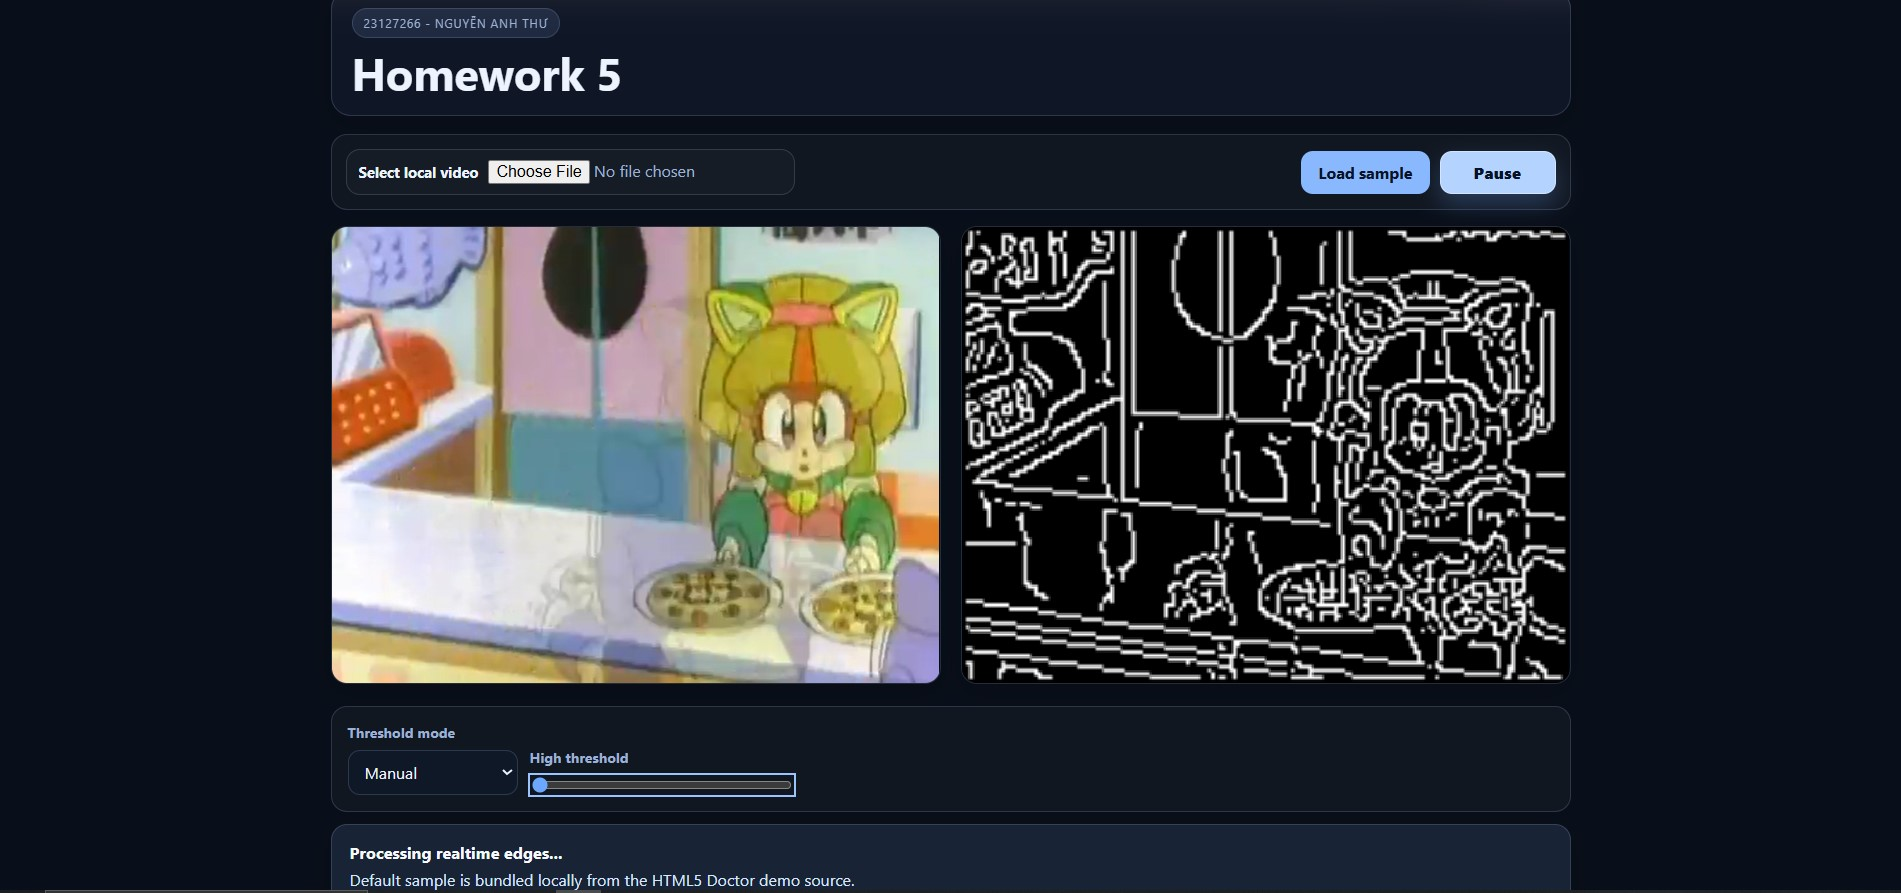
\includegraphics[width=0.95\linewidth]{img/result.PNG}
  \caption{Real-time edge output generated from the video stream.}
\end{figure}

\chapter{Implementation}
\section{Processing Flow}
\begin{figure}[!htbp]
  \centering
  \resizebox{0.95\textwidth}{!}{%
    \begin{forest}
      for tree={
        draw,
        rounded corners,
        align=center,
        fill=gray!6,
        grow'=east,
        s sep=5mm,
        l=10mm,
        parent anchor=east,
        child anchor=west,
      }
      [Video Input
        [Extract Current Frame
          [Grayscale
            [Separable Gaussian Blur
              [Sobel Gradients
                [Quantized Direction + Non-Maximum Suppression
                  [Hysteresis Thresholding
                    [Canvas Edge Output]
                  ]
                ]
              ]
            ]
          ]
        ]
      ]
    \end{forest}%
  }
  \caption{Real-time frame processing pipeline.}
\end{figure}

\section{Interface Structure}
The interface contains a local file picker, a sample-loading button, a play/pause button, a \texttt{video} element for the input stream, and a visible Canvas for the edge output. It also includes a threshold mode selector, a threshold slider, and status text for reporting the current processing state. Internally, an offscreen Canvas is used for intermediate pixel-level computation.

\section{Core Browser Functions}
The processing workflow is controlled by video playback events and a frame-synchronized rendering loop. The main browser and Canvas APIs used are:
\texttt{play()}, \texttt{pause()}, \texttt{addEventListener()}, \texttt{URL.createObjectURL()},
\texttt{getContext('2d')}, \texttt{drawImage()}, \texttt{getImageData()}, \texttt{putImageData()},
\texttt{clearRect()}, \texttt{requestAnimationFrame()}, and \texttt{cancelAnimationFrame()}.

\section{Frame Extraction}
The system does not process the raw video file directly. Instead, it processes the currently displayed frame. For each iteration, the current frame is copied from the \texttt{video} element to the internal processing Canvas using \texttt{drawImage()}, then converted into a pixel buffer through \texttt{getImageData()} for subsequent edge computation. Importantly, this internal Canvas runs at a reduced processing resolution controlled by \texttt{processingScale = 0.35}, after which the binary edge result is written back and upscaled onto the visible output Canvas.

\section{Edge Detection Pipeline}
The edge detector follows a compact Canny-style pipeline optimized for real-time execution:
\begin{enumerate}
  \item \textbf{Grayscale conversion:} RGB values are converted into intensity values using an integer approximation of the standard luminance formula.
  \item \textbf{Noise reduction:} a separable Gaussian blur with a 5-tap kernel is applied horizontally and vertically to suppress noise with low computational cost.
  \item \textbf{Gradient estimation:} Sobel operators are used to compute horizontal and vertical gradients, from which gradient magnitude and a 4-direction quantized orientation are obtained.
  \item \textbf{Non-maximum suppression:} local maxima are preserved along the gradient direction to produce thinner and more precise edges.
  \item \textbf{Thresholding with hysteresis:} the system supports both a manual high threshold and an adaptive high threshold derived from the mean gradient magnitude. The low threshold is computed as a fixed ratio of the high threshold. Strong edges are retained directly, while weak edges are preserved only if connected to strong responses in the 8-neighborhood.
\end{enumerate}

\section{Real-Time Scheduling}
The processing loop is driven by \texttt{requestAnimationFrame()} to remain synchronized with browser rendering. Redundant processing is reduced by skipping frames whose \texttt{currentTime} has not changed enough since the previous processed frame. For efficiency, the implementation also reuses preallocated typed buffers for grayscale, blur, gradient, suppression, classification, and hysteresis traversal.

\chapter{Limitations, Future Work, and Conclusion}
\begin{itemize}
  \item Performance depends on video resolution and device capability.
  \item Edge quality is sensitive to threshold selection and blur configuration.
  \item The implementation prioritizes responsiveness and portability over the accuracy of specialized vision libraries.
\end{itemize}

Future improvements include moving computation to \emph{OffscreenCanvas} or \emph{Web Workers}, and extending the parameter control strategy with more adaptive threshold selection.

In conclusion, this project demonstrates that real-time edge detection can be achieved efficiently in a browser using only HTML5 Video, Canvas, and client-side JavaScript. The implementation combines frame extraction, grayscale conversion, Gaussian smoothing, Sobel gradients, non-maximum suppression, and hysteresis thresholding in a fully local processing pipeline.